\chapter{Introducción a la energía solar}
\label{solar}

\section{El Sol}
El Sol es tautologicamente la fuente de energía electromagnética mas abundante y potente de nuestro sistema planetario, nuestro planeta Tierra se ubica en la galaxia de la Vía Láctea en uno de sus brazos espirales llamado el brazo de Orión, en este brazo se encuentra un sistema llamado Solar\cite{solar:1}, sistema que lleva su nombre por su estrella principal, El Sol.\\

En astronomía el Sol esta clasificado como una estrella del tipo espectral G2 y se encuentra ubicado en el centro del sistema solar. La luz emitida por el sol tarda 8 minutos y 19 segundos\cite{solar:2} en alcanzar el planeta Tierra y su energía constituye la fuente primordial del sustento de la vida basada en la fotosíntesis, es responsable del clima existente en nuestro planeta y de todas las condiciones de habitabilidad.\\

El sol se encuentra en una fase denominada secuencia principal, se formo aproximadamente hace 4.570 millones de años y se espera que continúe en la misma fase por otros 5000 millos de años mas.\\
Consecuencia de la reacciones termonucleares que se producen en el interior del sol, nuestro planeta recibe segundo a segundo cantidades muy grandes de energía, de manera sencilla el sol convierte cada segundo 564 millones de toneladas de Hidrógeno en 560 toneladas de Helio, esto quiere decir que aproximadamente 4 millones de toneladas de materia se convierten en energía que es expulsada al Universo, de la cual solo una pequeña porción es recibida por el planeta Tierra. En números la energía producida por el sol se calcula aproximadamente en $3,8 x {10}^{23} [kWatts]$\cite{solar:3}\\

La radiación solar medida en $W/{m}^{2}$, que inside en la atmósfera de nuestro planeta alcanza los $1395 W/{m}^{2}$ este valor se denomina la \textbf{Constante Solar} y es un valor medio entre el valor máximo del perihelio\gloss{Perihelio} y el valor mínimo del afelio\gloss{Afelio}.\\

\begin{figure}[h!]
        \centering
        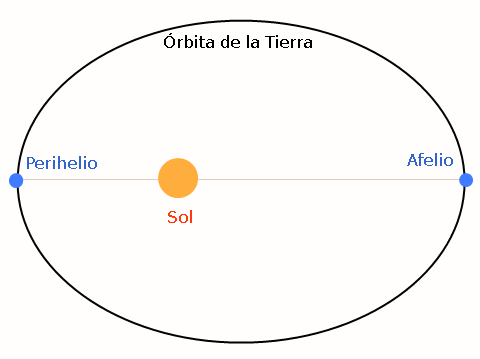
\includegraphics[scale=0.4]{images/afelioPerihelio}
        \caption{\tiny Esquema que muestra la orbita de la Tierra con respecto al Sol y muestra los puntos del Afelio y el Perihelio}
\end{figure}

El Sol no solo pertenece a la historia moderna de la humanidad, en la literatura se encuentran infinidad de referencias y escritos dedicados a esta grandiosa estrella que ilumina nuestro planeta Tierra, es solo en la actualidad y en la historia reciente que esta estrella es denominada como Sol pero para muchas culturas antiguas el Sol era una entidad muy importante, tanto así que para la cultura de la civilización egipcia representaba su deidad principal denominada Ra, en Latinoamérica se sabe que los Incas le llamaban Inti el cual era parte importante en ritos y sistemas de vida, los griegos representaban al sol de manera un poco mas compleja, este era un carro arrastrado por 4 caballos el cual era conducido por Helios. Y así podríamos seguir mencionando multitud de referencias a la historia antigua de la humanidad en donde este astro era considerado uno de los dioses centrales y mas importantes.\\ 

Como he mencionado en los párrafos anteriores el Sol produce enormes cantidades de energía y ha sido venerado durante toda la historia de la humanidad y prácticamente toda referencia que se tiene de este apunta a como este astro permite que la vida se desarrolle en nuestro planeta, debido a todas estas características es que el hombre siempre ha intentado beneficiarse de la cantidad de energía que llega a nuestro planeta. Los intentos y logros han sido diferentes dependiendo de la época y los desarrollos tecnológicos de la civilizaciones, pero podríamos coincidir en que todas las civilizaciones antiguas y modernas han intentado producir energía a partir de su radiación y de alguna manera todas lo han logrado pero el tema principal es con que nivel de eficiencia se ha conseguí esta tarea.\\

Para aprovechar esta energía, en la actualidad existen diversas tecnologías, ente las mas usadas están la conversión a energía eléctrica, la conversión a energía térmica o el aprovechamiento de viento producido por el calentamiento de masas de aire, entre muchas otras, cada tipo de conversión obtienen diferentes niveles de eficiencia y en su aprovechamiento influyen muchos factores, lamentablemente no es tema de esta memoria tratar estos temas en detalle, pero si nos enfocaremos un poco en la conversión a energía eléctrica.\\

\section{La radiación solar}
La Radiación emitida por el Sol viaja a través del espacio en forma de ondas electromagnética como toda onda posee una frecuencia y se puede clasifica de acuerdo a esta. El espectro de la radican solar se clasifica en tres grupos principales, la radiación UV, la Luz visible y la radiación Infrarroja, para los sistemas de producción de energía el espectro que mas interesa es el espectro de radiación UV ya que es el mas energético en comparación a los demás.

\begin{figure}[h!]
        \centering
        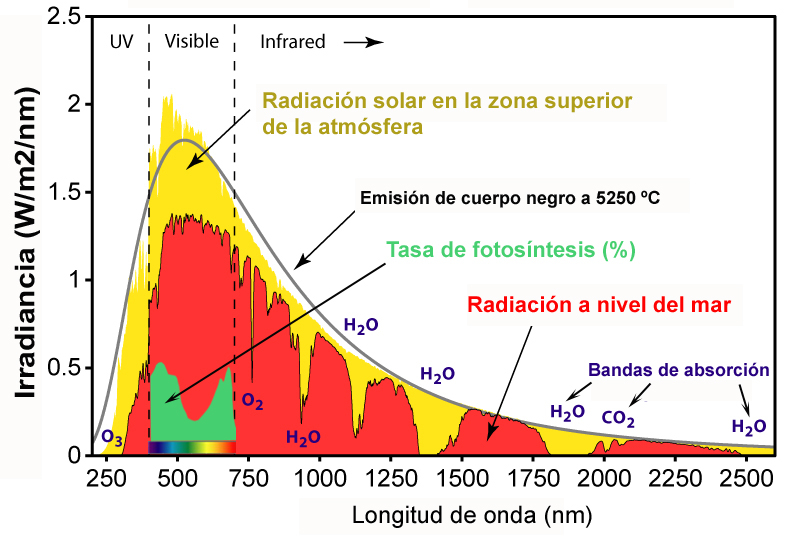
\includegraphics[scale=0.4]{images/espectroSolar}
        \caption{\tiny Gráfico de clasificación del espectro de la radiación solar\cite{recursoSolar:1}}
\end{figure}

Si medimos la radiación solar sobre la atmósfera del planeta obtendríamos lecturas cercanas a los 1350 $W/{m}^{2}$, este valor recibe el nombre de constante solar y es calculado como un valor medio entre la redición que recibimos en el periodo en que la Tierra esta mas cerca del sol y el valor en que la Tierra esta mas lejos del sol. El problema que se nos presenta en este punto es que la energía no puede ser captada desde el espacio sino desde la superficie terrestre y para llegar a esto la radiación proveniente del sol debe atravesar la atmósfera del planeta la cual tiene un grosor aproximado de 80 km y esta compuesta de gases principalmente de nitrógeno y oxigeno. Al calentarse estos gases producto de la redición producen entre algunos fenómenos los vientos y aportan a la formación de nubes, como consecuencia e esta absorción de energía sobre la superficie terrestre incide una cantidad de energía bastante menor a la medida en el espacio cercano al planeta.

\begin{figure}[h!]
        \centering
        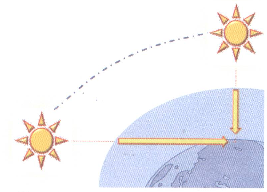
\includegraphics[scale=0.4]{images/espesorAtmosfera}
        \caption{\tiny Distancia que atraviesa la radiación en la atmósfera dependiendo del ángulo de incidencia\cite{recursoSolar:1}}
\end{figure}

Es debido a las condiciones climáticas y a la configuración química y física de la atmósfera que cada punto geográficos sobre la superficie terrestre recibirá diferentes cantidades de radiación. Tal como mencionábamos con anterioridad Chile presenta condiciones excepcionales en cuanto a la cantidad de radiación recibida en la superficie terrestre. Estudios realizados en nuestro país por diversas instituciones estiman que en el norte de nuestro país es posible recibir mas de 1000 $W/{m}^{2}$

La radiación que inside en la superficie terrestre se denomina GI\gloss{gi} esta radiación tiene 3 componentes, DNI\gloss{dni}, Radiación difusa\gloss{rd} y la radiación reflejada. $$ GI = DNI + Rdifusa + Rreflejada $$

\begin{figure}[h!]
        \centering
        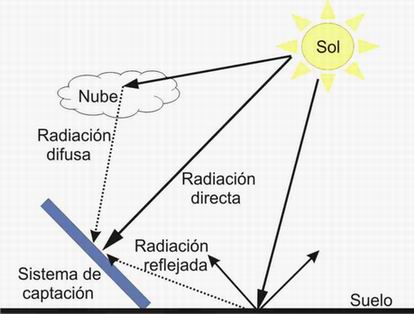
\includegraphics[scale=0.4]{images/radiacionDescompocicion}
        \caption{\tiny Descomposición de la radiación solar\cite{recursoSolar:1}}
\end{figure}

De esta definición derivan dos tipos de radiación que resultan relevantes para la producción energética fotovoltaica, la primera de ellas es la Radiación Global Horizontal\gloss{ghi}(GHI) y la Radiación Directa Normal\gloss{dni}. La GHI es la radiación medida en el plano horizontal a una superficie dada sobre la tierra mientras que la DNI es la radiación medida en dirección normal al Sol. $$ GHI = DNI cos \theta + Rdifusa + Rreflejada $$

(foto)

\section{Energía fotovoltaica}
Se llama luminosidad solar a la energía emitida por el Sol en un momento de tiempo dado, ahora bien es posible calcular la luminosidad que recibe la tierra en un momento puntual utilizando los valores de la constante solar definida en la sección anterior. Esto se hace considerando que la luminosidad disminuye con la distancia entre el sol y la tierra y la superficie del planeta Tierra, este calculo nos dice que nuestro planeta recibe  $3,65 x {10}^{23} KW$ instantáneos. Esta cantidad de energía es equivalente a 4000 veces toda la producción energética del planeta en una año\\

Para entender de manera mas sencilla debemos explicar la diferencia entre el concepto de potencia y energía. Cuando hablamos de potencia queremos decir que cierta cantidad de ...\\

Chile posee características naturales de excelencia en cuanto a la cantidad de energía solar recibida desde el espacio, estas condiciones posicionan a nuestro país dentro de la localidades con mejor componente solar en el planeta para la producción de energía fotovoltaica, a pesar de estas buenas condiciones nuestro país no ha desarrollado ni aplicado las tecnologías necesarias para aprovechar de buena manera esta ventaja.\\

La matriz energética de Chile tiene una potencia instalada de $15.558 MW$\cite{matrizEnergia:1} los cuales el 64\% es energía termoeléctrica, un 35\% es energía hidroeléctrica y 1\% corresponde a energía eólica. Del 64\% de energía termoeléctrica se considera la producida por el gas natura, el carbón y el petroleo. Adicionalmente de toda la matriz el 68\% es importada\cite{colegioIng:1}, esto quiere decir que nuestro país al año 2010 es incapaz de autoabastecerse enérgicamente, dependemos de la cantidad de energía que este disponible para la viene desde el exterior, esto suena un poco ridículo considerando que en el país tenemos uno de los mejores recursos solares del mundo.\\

A pesar de que la tecnología no se haya desarrollado en nuestro país, existen importantes experiencias, en investigación y aplicación en donde hemos sido pioneros, a pesar de esto han sido otros países especialmente europeos quienes han recogido estas investigaciones y han potenciado el desarrollo de esta tecnología, países como España y Alemania que hoy en día son pioneras en cuanto a la producción e investigación en energías renovables no convencionales.\\

una vivienda promedio en chile consume....\\

Los 3 usos principales de la energía en los hogares de chile son, agua caliente sanitaria, cocción de alimentos y calefacción, el consumo medio nacional de una vivienda es de 10.232 KWh/año incluyendo todos los tipos de energía utilizados e la vivienda, ahora bien si eliminamos la leña consumida en el sur de chile la media anual seria de 4.470 KWh/año esto debido al bajo precio de la leña y el confort térmico que entrega.
calculo aproximado....\\

http://www.edicionesespeciales.elmercurio.com/destacadas/detalle/index.asp?idnoticia=20110518718980\&idcuerpo=962\\
http://www.chilerenuevaenergias.cl/index.php?option=com\_k2\&view=item\&layout=item\&id=10\\
http://www.ecopotencia.com/vivienda.html\\

costos ....\\
http://nuevopolitico.bligoo.cl/tag/matrizenergeticadechileano2010\\

\section{Sistemas fotovoltaicos}
Para capturar la radiación solar incidente en la superficie terrestre y transformarla a energía eléctrica se debe utilizar un conjunto de componentes de hardware eléctricos, el sistema mas básico consta de un panel solar, un inversor y una batería. Uno de los grandes problemas del sector energético ha sido durante mucho tiempo el como se debe almacenar la energía producida y los sistemas fotovoltaicos no están ajenos a este problema principalmente porque la radiación solar no es constante durante el día ni mucho menos durante el año, mas aun un sistema fotovoltaico solo producirá energía eléctrica durante las horas de sol o de día, mientras los fotones de las ondas electromagnéticas provenientes del sol existen átomos de silicio.

\subsection{Paneles solares}
Las primeras referencias que se tienen de paneles solares son del año 1954 cuando se descubrió que el silicio con ciertas impurezas era muy sensibles a la luz. Uno de los datos interesantes aquí es que el silicio es el segundo elemento mas abundante en la Tierra después del Oxigeno con un 28\% de la masa total.
\\

Los primero paneles solares que se fabricaron solo tenia una eficiencia el 4.5\% sin embargo fue durante la segunda mitad de la década del 1950 cuando esta tecnología empezó a desarrollarse con mas fuerzas debido a la carrera espacial entre EEUU y la Unión Soviética durante 1950 y 1980. Actualmente la eficiencia de los mejores paneles solares alcanzan alrededor del 30\%.\\

Los paneles solares están fabricado por una gran cantidad de pequeñas celdas hechas de silicio, además de algunos otros materias como los marcos y los protectores en menor proporción. El silicio se encuentra en la cortesía terrestre sin embrago no se encuentra puro de manera natura y es necesario someterlo a diferentes procesos químico para purificarlo y obtener cristales. Durante mucho tiempo este proceso fue muy caro, sin embargo hoy en día esto tiene a reducirse de manera significativa gracias al desarrollo de la tecnología y a la masificación del mercado. A pesar de esto la energía requerida para purificar el silicio para la formación de paneles es bastante alta y un panel debe funcionar por algunos años antes de recuperar la energía utilizada en su confección.\\

Los países que actualmente producen la mayor cantidad de celdas de silicio se representan en la siguiente gráfica:\\

(foto)\\

Para que un panel solar genere energía eléctrica varios procesos físicos y químicos deben ocurrir, como mencionaba en el primer párrafo el silicio es altamente sensible a la luz, esta propiedad causas que cuando un fotón choque con una molécula de silicio los electrón de esta salten de una molécula a otra, sin embargo para aprovechar la energía de esta reacción es necesario que la celda fotovoltaica tenga una configuración especial, las moléculas de silicio deben estar separadas por una membrana unidireccional que permita que los electrones circulen solo en una dirección, actuando como un diodo.\\

(foto)\\

Para producir una diferencia de potencial elevada es necesario juntar muchas celdas fotovoltaica conectadas en serie, además para lograr una corriente que sea capas de encender equipos eléctricos es necesario combinar estos arreglos en serie con otros arreglos en serie conectados en paralelo.\\

(foto)\\

Actualmente existen 4 tipos de paneles solares, o aplicaciones de silicio fotovoltaicas.\\
\subsubsection{Silicio monocristalino}
\subsubsection{Silicio Policristalino}
\subsubsection{Silicio amorfo}
\subsubsection{Silicio de capa fina}

\section{las leyes en chile y posibles modelos de negocio}
sistemas distribuidos...

